\chapter{金属材料机械性能测量:拉伸}
\section{实验目的}
\begin{enumerate}
    \item 了解电子万能试验机的基本结构、工作原理及使用方法;
    \item 观察拉伸时所表现的各种现象;
    \item 观察低碳钢和铸铁的断口特征,辨别两种材料的力学特征;
    \item 通过低碳钢和铸铁的应力-应变曲线,评价二者的力学性能,掌握金属材料屈服强度,抗拉强度,断裂伸长率和断面收缩率的测定方法。
\end{enumerate}
\section{实验原理}%简单描述,含必要的公式和附图;
\subsection{低碳钢拉伸的应力-应变曲线及特征参数}
\subsubsection{低碳钢拉伸的应力-应变曲线}
低碳钢是塑性材料的典型代表性材料,对于低碳钢试样,在受拉伸过程中,如\fgref{fig:A6.1} 所示应力-应变曲线,可以观察到试样经历四个典型的变形阶段:弹性变形阶段,屈服阶段,均匀塑性变形阶段(强化阶段),局部塑性变形阶段(颈缩阶段),伴随着应力-应变曲线上存在不同的特征点。
\begin{figure}[!ht]
    \begin{floatrow}\centering
        \ffigbox{\caption{低碳钢的拉伸曲线(R-e 曲线)}\label{fig:A6.1}}{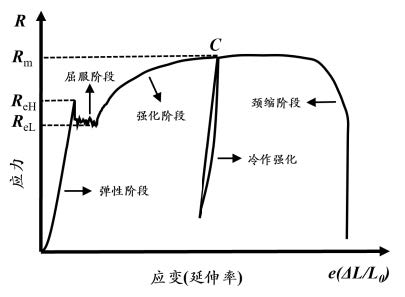
\includegraphics[height=50mm]{img/A6/1.jpg}}
        \ffigbox{\caption{铸铁的拉伸曲线}\label{fig:A6.2}}{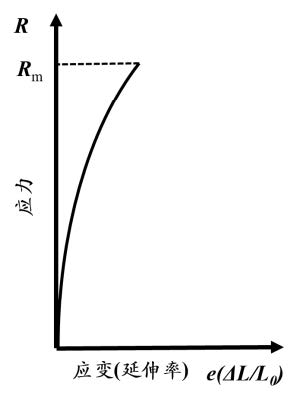
\includegraphics[height=50mm]{img/A6/2.jpg}}
    \end{floatrow}
\end{figure}
\subsubsection{铸铁的应力-应变曲线}
铸铁是典型的脆性材料,铸铁的拉伸变形无屈服现象和缩颈现象,进行非常小的塑性变形后在较小的应力作用下就可被拉断,且突然断裂。拉断后铸铁的延伸率通常很小,约为 0.5\%。\fgref{fig:A6.2} 为铸铁典型的应力-应变曲线,由图可见,铸铁的应力-应变曲线没有明显的直线部分。铸铁拉断前承受的最大应力值为其被拉伸的强度极限,定义为铸铁的抗拉强度。
\subsection{相关概念基本定义及计算公式}
\noindent 弹性模量:在应力-应变曲线上,应力低于弹性极限的范围内,应力与应变的比值,表达式为:\linebreak $E =\displaystyle \frac{\sigma}{\varepsilon}$ ,$\sigma$ 为应力,$\varepsilon$ 为应变。\\
上屈服强度 $R_{eH}$:试样发生屈服时应力下降时达到的最大值。\\
下屈服强度 $R_{eL}$:试样屈服期间屈服平台上不计初始屈服瞬时效应的最低应力点。\\
抗拉强度 $R_m$:试样缩颈前所达到的最大应力值。\\
原始标距 $L_0$:试样初始状态,夹头内用于测试的等截面积的试样部分的长度。\\
断后标距 $L_u$:实验被拉断后,将试样断口处紧密对接,初始标线内的总长度。\\
断后延伸率 $\delta$:试样拉断后,试样原始标线之间的伸长量和原始标距之比,$\delta = \displaystyle\frac{L_u-L_0}{L_0}\times 100\%$。\\
断面收缩率 $\psi$:试样拉断后,断口处横截面积的最大缩小量与原始标距内截面积之比,\linebreak $\psi = \displaystyle\frac{L_0-L_u}{L_0}\times 100\%$。
\section{实验仪器}%规格及参数
电子万能试验机,控制微机,游标卡尺,YYU-25/50 电子引伸计,低碳钢标准试样,铸铁标准试样。
\section{实验过程}%简述主要过程和实验内容
\begin{enumerate}
    \item 首先,在装夹试样前,标记待测试样的原始标距 $L_0$。选取待测试样夹头内部变形部分偏中间位置,在此处不同位置处选择3~5个截面,用游标卡尺在每个截面相互垂直的两个方向上分别测量一次该截面的直径,对所测量的所有截面直径求平均值即可视为待测试样拉伸之前的直径,记为 $d_0$,之后在待测试样夹头中间变形部分,以其变形部分的中点为中心,左右各选取 $5d_0$ 共 $10d_0$ 的长度,在端点处做标记,标记内即为待测试样的原始标距 $L_0$。
    \item 检查并确认电子万能试验机和计算机已连接。之后打开万能电子试验机,旋转红色急停旋钮使其弹起。
    \item 安装拉伸模具。
    \item 装夹试样。
    \item 装夹引伸计(低碳钢拉伸)。
    \item 编辑实验方案进行并进行测量。
    \item 进行测试
    \item 测量断后试样尺寸
    \item 保存数据,作图并分析待测试样各力学性能参数指标。
    \item 测量铸铁的拉伸曲线。
    \item 根据测量的低碳钢和铸铁的拉伸曲线,分析和判断两类金属材料的力学性能和各性能指标参数。
\end{enumerate}
\section{实验数据}
\subsection{尺寸数据}
\begin{table}[!ht]
    \caption{拉伸试样拉伸前几何尺寸测量数据}
    \begin{tabular}{*{9}{c}}\toprule
        & \multicolumn{2}{c}{直径 1} & \multicolumn{2}{c}{直径 2} & \multicolumn{2}{c}{直径 3} & \multirow[c]{2}{*}{$d_0$} & \multirow[c]{2}{*}{$L_0$} \\
        & 测量 1 & 测量 2 & 测量 1 & 测量 2 & 测量 1 & 测量 2 & & \\ \midrule
        低碳钢 & 4.82 & 4.82 & 4.84 & 4.86 & 4.92 & 4.94 & 4.867 & 48.67 \\ 
        铸铁 & 4.94 & 4.96 & 5.02 & 5.04 & 5.02 & 5.00 & 4.997 & 49.97 \\ \bottomrule
    \end{tabular}
\end{table}

\begin{table}[!ht]
    \caption{拉伸试样拉伸后几何尺寸测量数据}
    \begin{tabular}{*{10}{c}}\toprule
        & \multicolumn{6}{c}{断后标距} & \multicolumn{3}{c}{最小直径} \\
        & 测量 1 & 测量 2 & 测量 3 & 测量 4 & 测量 5 & 平均值 & 测量 1 & 测量 2 & 平均值 \\ \midrule
        低碳钢 & 60.12 & 59.72 & 59.70 & 60.06 & 59.72 & 59.864 & 2.68 & 2.70 & 2.69  \\ 
        铸铁 & 53.30 & 52.76 & 52.76 & 53.18 & 53.02 & 53.004 & 4.88 & 4.86 & 4.87  \\ \bottomrule
    \end{tabular}
\end{table}
\subsection{数据绘制}
\begin{figure}[!ht]
    \caption{低碳钢拉伸应力-应变曲线}
    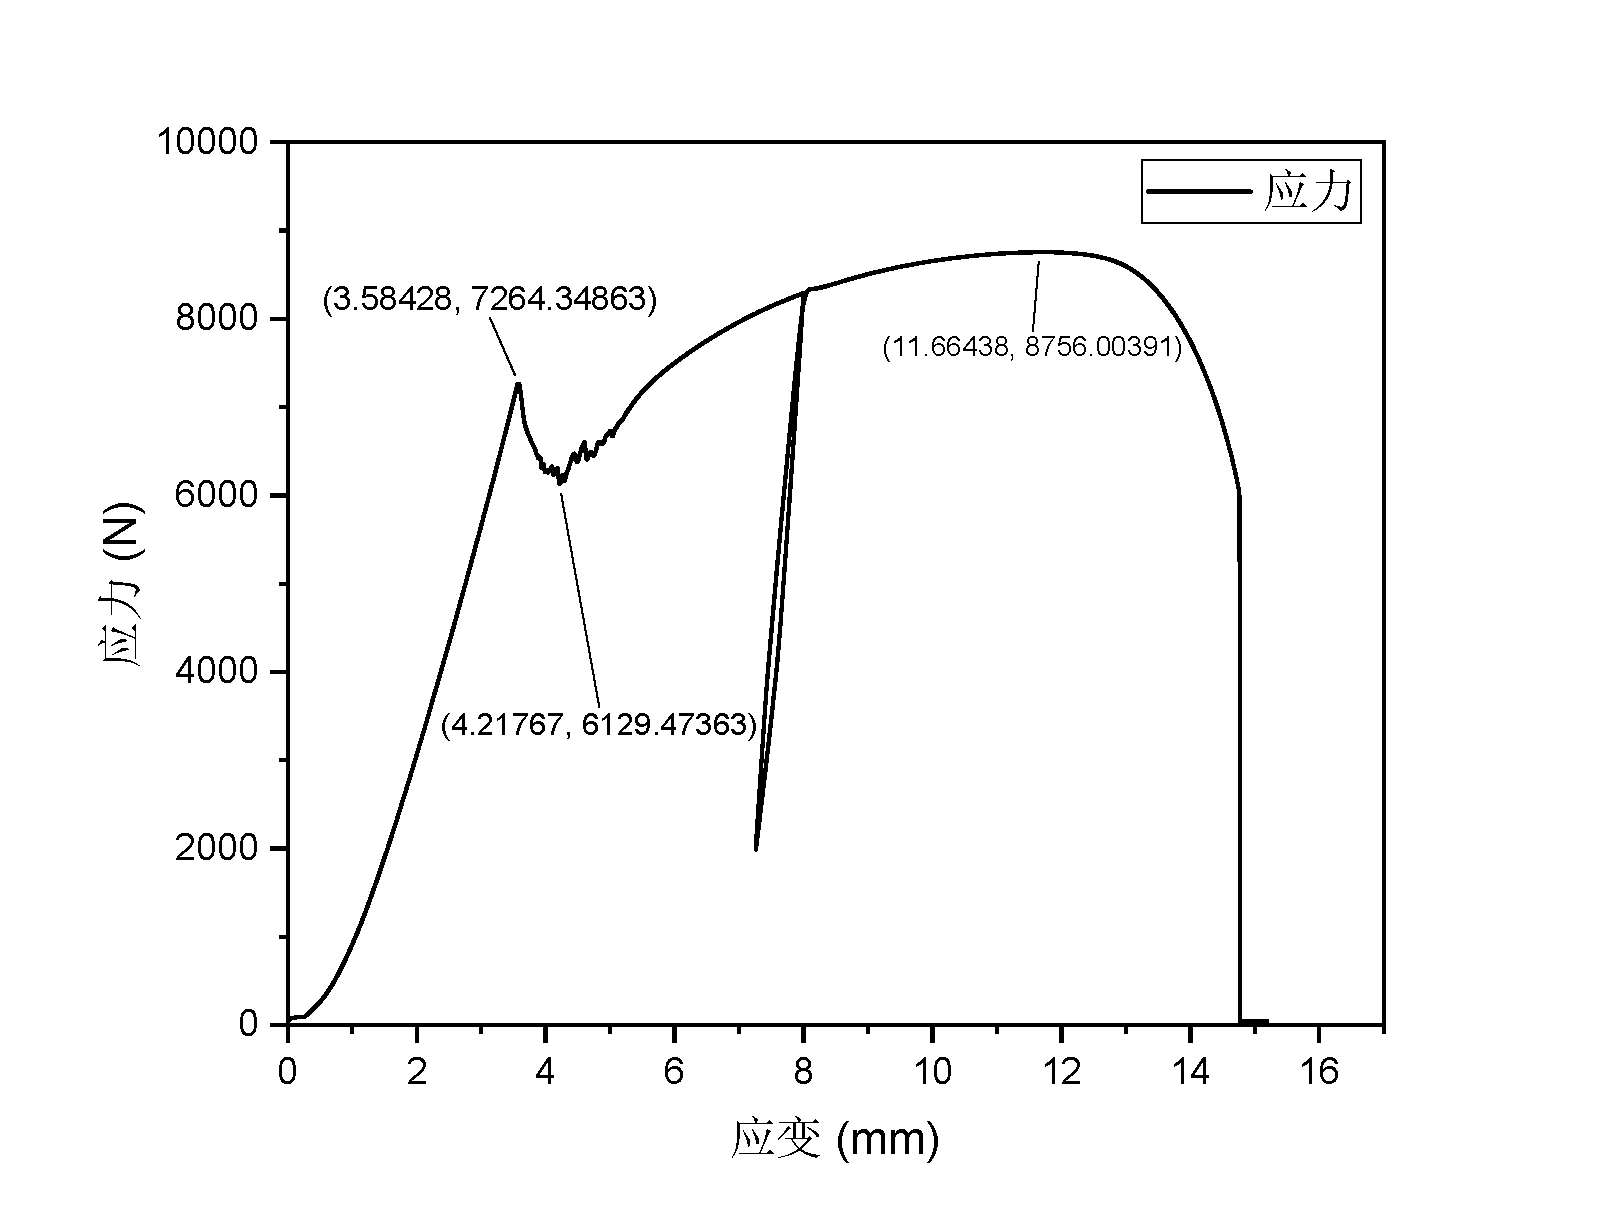
\includegraphics[width=0.6\textwidth]{img/A6/steelPull.pdf}
\end{figure}\newpage
\begin{figure}[!ht]
    \caption{铸铁拉伸应力-应变曲线}
    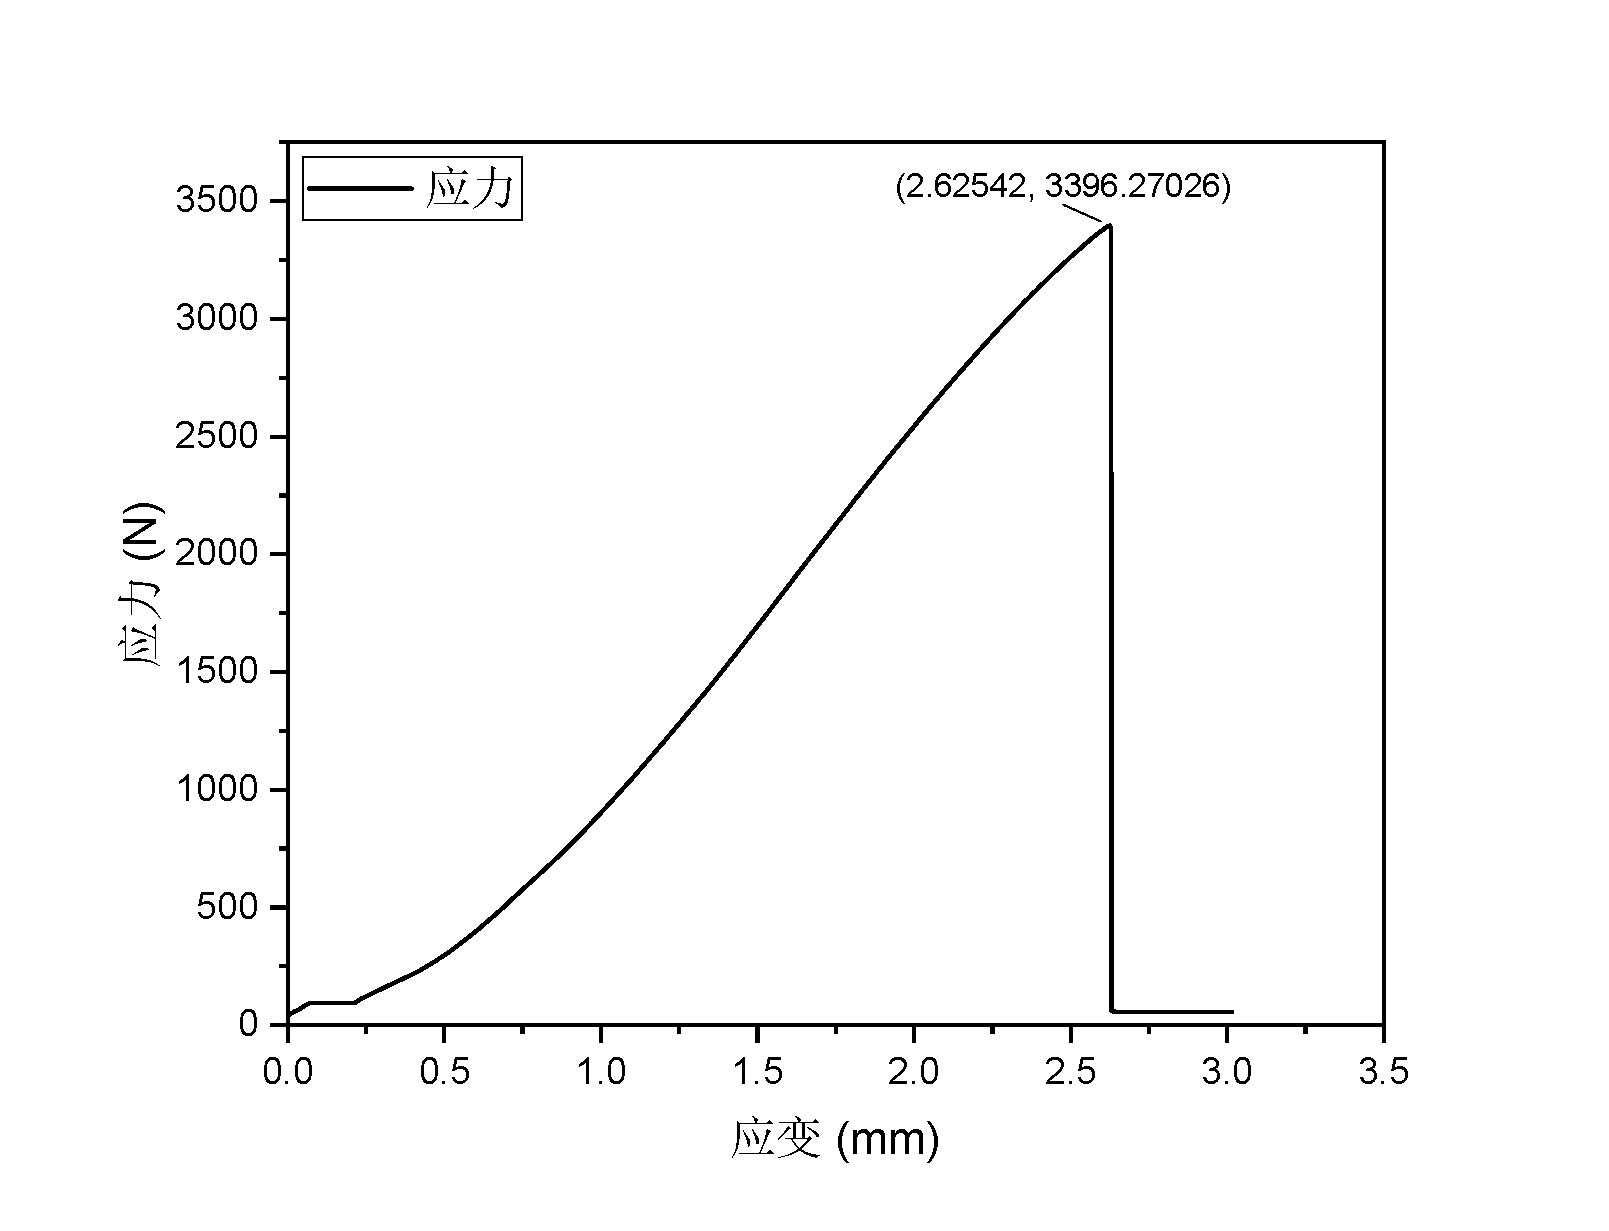
\includegraphics[width=0.6\textwidth]{img/A6/ironPull.pdf}
\end{figure}
\subsection{数据计算}
\subsubsection{低碳钢}
\noindent 断后延伸率
\begin{equation}
    A_1=\frac{L_u-L_0}{L_0}\times 100\%=\frac{59.864 - 48.67}{48.67}\times 100\%=23.000\%
\end{equation}
断后收缩率
\begin{equation}
    Z_1=\frac{S_0-S_u}{S_0}\times 100\%=\frac{d_0^2-d_u^2}{d_0^2}\times 100\%=\frac{4.867^2-2.68^2}{4.867^2}\times 100\% = 69.452\%
\end{equation}
上屈服强度
\begin{equation}
    R_{eH1}=\frac{F_{eH1}}{S_{0}}=\frac{4 F_{eH1}}{\pi d_{0}^2}=\frac{4\times 7264.34863}{\pi(4.867\times 10^{-3})^{2}}=\SI{3.90467d8}{\Pa}
\end{equation}
下屈服强度
\begin{equation}
    R_{eL1}=\frac{F_{eL1}}{S_{0}}=\frac{4 F_{eL1}}{\pi d_{0}^2}=\frac{4\times 6129.47363}{\pi(4.867\times 10^{-3})^{2}}=\SI{3.29466d8}{\Pa}
\end{equation}
抗拉强度
\begin{equation}
    \sigma_1=\frac{F_1}{S_{0}}=\frac{4 F_1}{\pi d_{0}^2}=\frac{4\times 8756.00391}{\pi(4.867\times 10^{-3})^{2}}=\SI{4.70645d8}{\Pa}
\end{equation}
\subsubsection{铸铁}
\noindent 断后延伸率
\begin{equation}
    A_2=\frac{L_u-L_0}{L_0}\times 100\%=\frac{53.004 - 49.97}{49.97}\times 100\%=6.072\%
\end{equation}
断后收缩率
\begin{equation}
    Z_2=\frac{S_0-S_u}{S_0}\times 100\%=\frac{d_0^2-d_u^2}{d_0^2}\times 100\%=\frac{4.997^2-4.87^2}{4.997^2}\times 100\% = 5.018\%
\end{equation}
抗拉强度
\begin{equation}
    \sigma_2=\frac{F_2}{S_{0}}=\frac{4 F_2}{\pi d_{0}^2}=\frac{4\times 3396.27026}{\pi(4.997\times 10^{-3})^{2}}=\SI{1.73178d8}{\Pa}
\end{equation}
计算结果汇总得到表 \ref{fig:A6.pull}
\begin{table}[!ht]
    \caption{拉伸实验计算结果}\label{fig:A6.pull}
    \begin{tabular}{|c|*{8}{m{3.3em}|}} \hline
        试样 & \multicolumn{5}{c|}{低碳钢} & \multicolumn{3}{c|}{铸铁} \\ \hline
        数据名称 & 上屈服强度 (\unit{\MPa}) & 下屈服强度 (\unit{\MPa}) & 抗拉强度 (\unit{\MPa}) & 断后延伸率 (\%) & 断后收缩率 (\%) & 抗拉强度 (\unit{\MPa}) & 断后延伸率 (\%) & 断后收缩率 (\%) \\ \hline
        数值 & 390.467 & 329.466 & 470.645 & 23.000 & 69.452 & 173.178 & 6.072 & 5.018 \\ \hline
    \end{tabular}
\end{table}

\section{结果分析}
\subsection{数据分析}
实验测量绘制的低碳钢拉伸曲线主要分为五个阶段,与理论图像的曲线非常相符,说明本次实验真实反映了低碳钢在拉伸应力作用下的形变过程。同时,我们可以从测得的铸铁拉伸曲线中看出,铸铁在较小应力下就发生了断裂,与理论相符。但有一点值得注意,理论的铸铁延伸率参考值为 0.4\%,而本实验计算出的延伸率为 6.072\%。这可能是因为断后拼接测量时拼接的缝隙较大,导致断后标距较实际值偏大。拉伸时受力不均也会导致样品发生滑移,使得断后标距偏大。
\subsection{误差分析}
\subsubsection{系统误差}
\begin{enumerate}
    \item 环境:实验当天的温度、湿度所带来的误差。查阅资料得知,温度、湿度会在一定程度下影响材料的力学性质,进而影响实验测量。
    \item 仪器:诸如测量数据时的精度,加载应力时的均匀程度之类仪器本身的误差,以及用游标卡尺测量直径和长度时精度带来的误差。
    \item 试样:不同的试样中的组成成分差异带来的误差。
\end{enumerate}
\subsubsection{偶然误差}
\begin{enumerate}
    \item 读数:在用游标卡尺测量试样的长度和直径时,可能会由于估读而产生读取数据的误差。
    \item 计算:在对数据进行处理分析时,可能会由于四舍五入而产生计算的误差。
\end{enumerate}
\section{思考题}
\begin{enumerate}
    \item \thinking{比较低碳钢和铸铁的拉伸曲线,讨论其差异。}{
        \begin{enumerate}
        \item 强度:比较本实验低碳钢和铸铁的拉伸曲线可知,低碳钢的抗拉强度为 \SI{470.645}{\MPa},铸铁的抗拉强度为 \SI{173.178}{\MPa}。由此可见,低碳钢通常比铸铁具有更高的拉伸强度。这是因为低碳钢具有更均匀的结晶结构和较少的缺陷,使其具有更高的抗拉性能。
        \item 延展性:低碳钢通常比铸铁具有更好的延展性。根据曲线可以看出,低碳钢的图像出现了一段水平锯齿状的曲线,这意味着受力时低碳钢发生了塑性变形而不会立即断裂。相比之下,铸铁则没有塑性变形阶段,更容易发生脆性断裂。
        \end{enumerate}}
    \item \thinking{低碳钢在拉伸过中可分为几个阶段,各阶段有何特征?}{
        \begin{enumerate}
        \item 弹性阶段:在这个阶段,材料受到外力时,会产生应力,但这个应力与应变成正比关系,即满足胡克定律。此时,材料发生的变形是完全可逆的,材料会在去除外力后恢复原状。
        \item 屈服阶段:随着应力的增加,材料达到一定的应力值后,开始出现非线性变形,即发生塑性变形,这一点称为屈服点。在屈服点之后,材料会出现永久性的变形,而不是完全恢复到原来的状态。
        \item 屈服后硬化阶段:在超过屈服点后,材料会经历硬化阶段。尽管材料仍然发生塑性变形,但其抗拉强度继续增加,这是由于在变形过程中形成了更多的位错,导致材料内部发生局部加固。
        \item 颈缩阶段:当材料达到一定的应力值时,开始在局部区域发生颈缩,这是因为材料在这些区域发生了更多的塑性变形,导致其截面积减小。在这个阶段,材料的应力基本上保持不变,但变形集中在颈缩区域。
        \item 断裂阶段:最终,材料达到其最大承载能力,无法再继续承受应力。在这个阶
        段,材料会发生断裂,使其失去了结构完整性。
        \end{enumerate}}
    \item \thinking{何谓“冷作硬化”现象?此现象在工程中如何运用?}{“冷作硬化”是指在常温下对金属材料进行塑性变形(例如拉伸、压缩、弯曲等),导致其硬度、强度和抗拉弯性能提高的现象。这种硬化是由于金属晶粒在变形过程中发生滑移和再结晶等微观结构变化所致。\par
    在工程中,冷作硬化现象可以用于改善材料的机械性能,例如增加金属的强度、硬度和抗拉弯性能。这种方法可以用于生产高强度、高硬度的零件或制品,如汽车零件、建筑结构、航空航天部件等。冷作硬化还可以用于调节金属材料的弹性模量和导电性能等特性,使其更适用于特定的工程应用。但过度的冷作硬化可能会导致材料变脆,降低其韧性和抗冲击性能,因此在工程设计中需要权衡利弊。}
\end{enumerate}
\chapter{金属材料机械性能测量:压缩}
\section{实验目的}
    \begin{enumerate}
        \item 测定低碳钢在压缩时的名义屈服强度 $R_\text{pc0.2}$;
        \item 测定铸铁在压缩时的强度极限 $R_m$;
        \item 观察上述材料在压缩时的变形及破坏形式,并分析其破坏原因;
        \item 比较塑性材料与脆性材料的力学性能及特点。
    \end{enumerate}
\section{实验原理}%简单描述,含必要的公式和附图;
    \subsection{低碳钢}
        低碳钢为塑性材料,其压缩曲线($F$-$\Delta L$ 曲线)如\fgref{fig:A6.4} 所示,开始加载时,力-变形曲线呈直线上升,此时材料服从胡克定律。当载荷达到一定值以后,随载荷增加变形加快,不再为线性关系,但试样无明显屈服现象。随载荷进一步增大,曲线逐渐向上弯曲。这是因为随着塑性变形的迅速增长,试样横截面积逐渐增大,增加了承载能力,同时纵向变形速度下降,从而导致力-变形关系曲线上翘。
        \begin{figure}[!ht]
            \subfloat[\mbox{}]{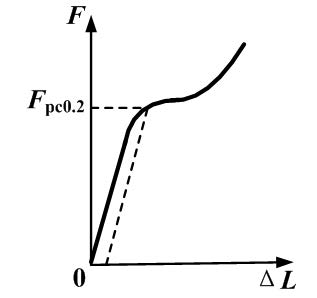
\includegraphics[height=35mm]{img/A6/4.jpg}\label{fig:A6.4}}\hspace{10mm}
            \subfloat[\mbox{}]{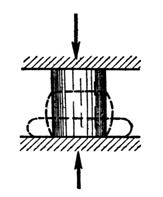
\includegraphics[height=35mm]{img/A6/5.jpg}}
            \caption{低碳钢压缩图}
        \end{figure}
        \subsection{铸铁}
            铸铁为脆性材料,其压缩曲线在开始时接近直线。随载荷增加曲率逐渐增大,最后至破坏,破坏后试件的断面法线方向与轴线夹角 $\alpha$ 大约为 $45^\circ$-$55^\circ$。\par
            如\fgref{fig:A6.5a} 所示,铸铁没有屈服极限,只有在最大载荷 $F_m$ 下测出的强度极限 $R_m$。铸铁的抗压强度极限比它的抗拉强度极限高 $3\sim4$ 倍。其它脆性材料,如混凝土、石料等的抗压强度也远高于相应材料的抗拉强度。
            \begin{figure}[!ht]
                \subfloat{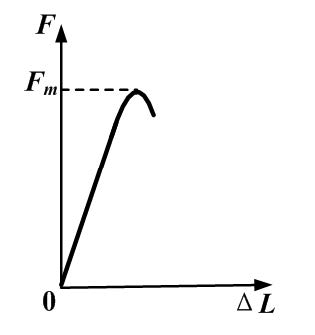
\includegraphics[height=35mm]{img/A6/6.jpg}}\hspace{10mm}
                \subfloat{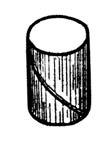
\includegraphics[height=35mm]{img/A6/7.jpg}}
                \caption{铸铁压缩图}\label{fig:A6.5a}
            \end{figure}
\
\section{实验仪器}%规格及参数
    \begin{enumerate}
        \item 实验所采用的设备及工具与拉伸实验相同。
        \item 压缩模具。
        \begin{figure}[!ht]
            \caption{压缩模具}
            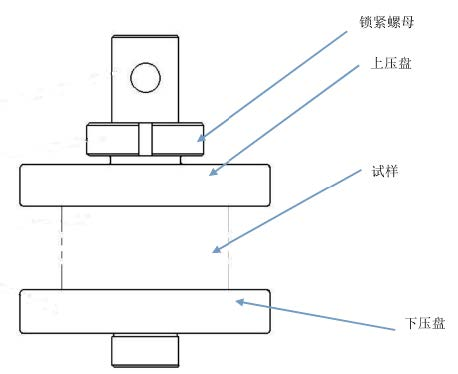
\includegraphics[height=40mm]{img/A6/3.jpg}
        \end{figure}
    \end{enumerate}
\section{实验过程}%简述主要过程和实验内容
    \begin{enumerate}
        \item 用游标卡尺在互相垂直方向,两次测量金属材料试件的直径,取其平均值为 $d_0$(用于计算试件原始截面面积 $S_0$),同时测量试件高度 $h$(测一次即可)。
        \item 打开设备
        \item 设置试验方案
        \item 装夹试样
        \item 开始测试
        \item 实验结束,将横梁上升,取出被测试样;点击“预览”生成测试结果报告并保存;
    \end{enumerate}
\newpage
\section{实验数据}
    \subsection{尺寸数据}
    \begin{table}[!ht]
        \caption{压缩试样压缩前几何尺寸测量数据}
        \begin{tabular}{*{4}{c}}\toprule
            & \multicolumn{3}{c}{断后标距}\\
            & 测量 1 & 测量 2 & 平均值 \\ \midrule
            低碳钢 & 3.90 & 3.88 & 3.89 \\ 
            铸铁 & 3.88 & 3.88 & 3.88 \\ \bottomrule
        \end{tabular}
    \end{table}
    \subsection{数据绘制}
    \begin{figure}[!ht]
        \caption{低碳钢压缩应力-应变曲线}
        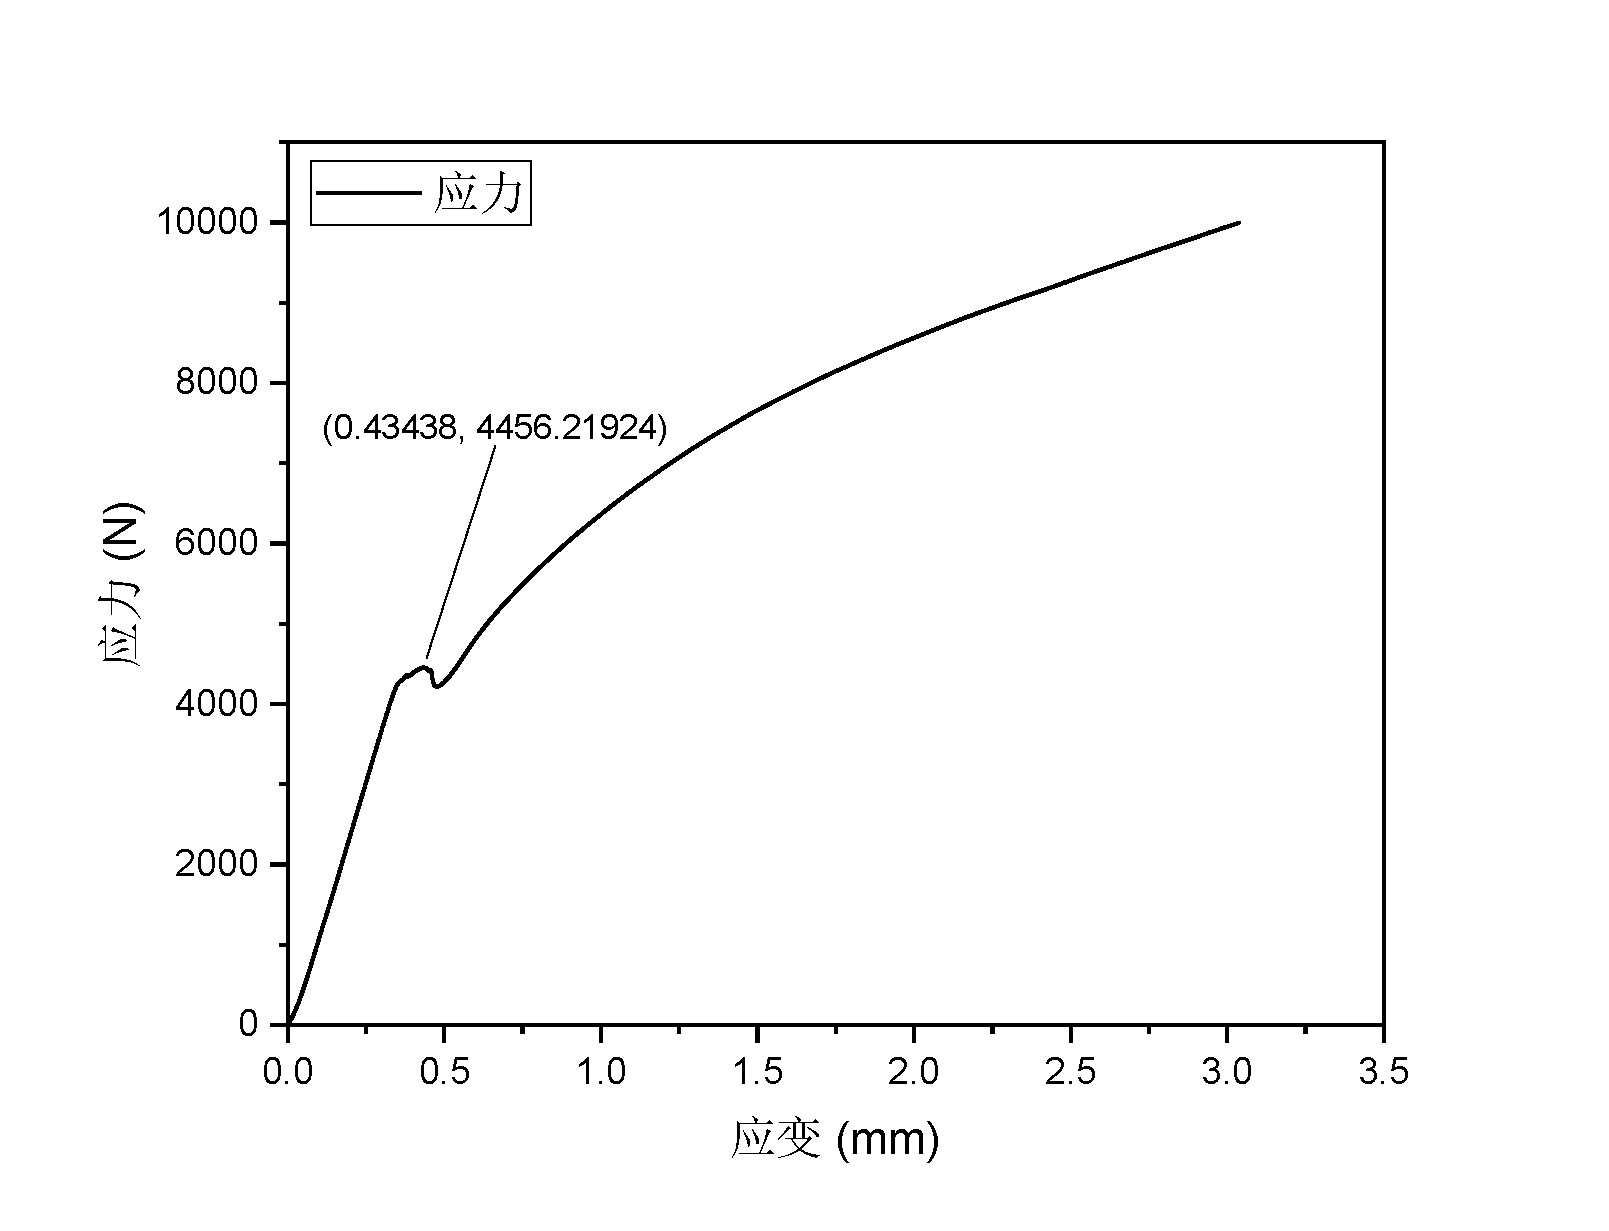
\includegraphics[width=0.5\textwidth]{img/A6/steelPush.pdf}
    \end{figure}
    \begin{figure}[!ht]
        \caption{铸铁压缩应力-应变曲线}
        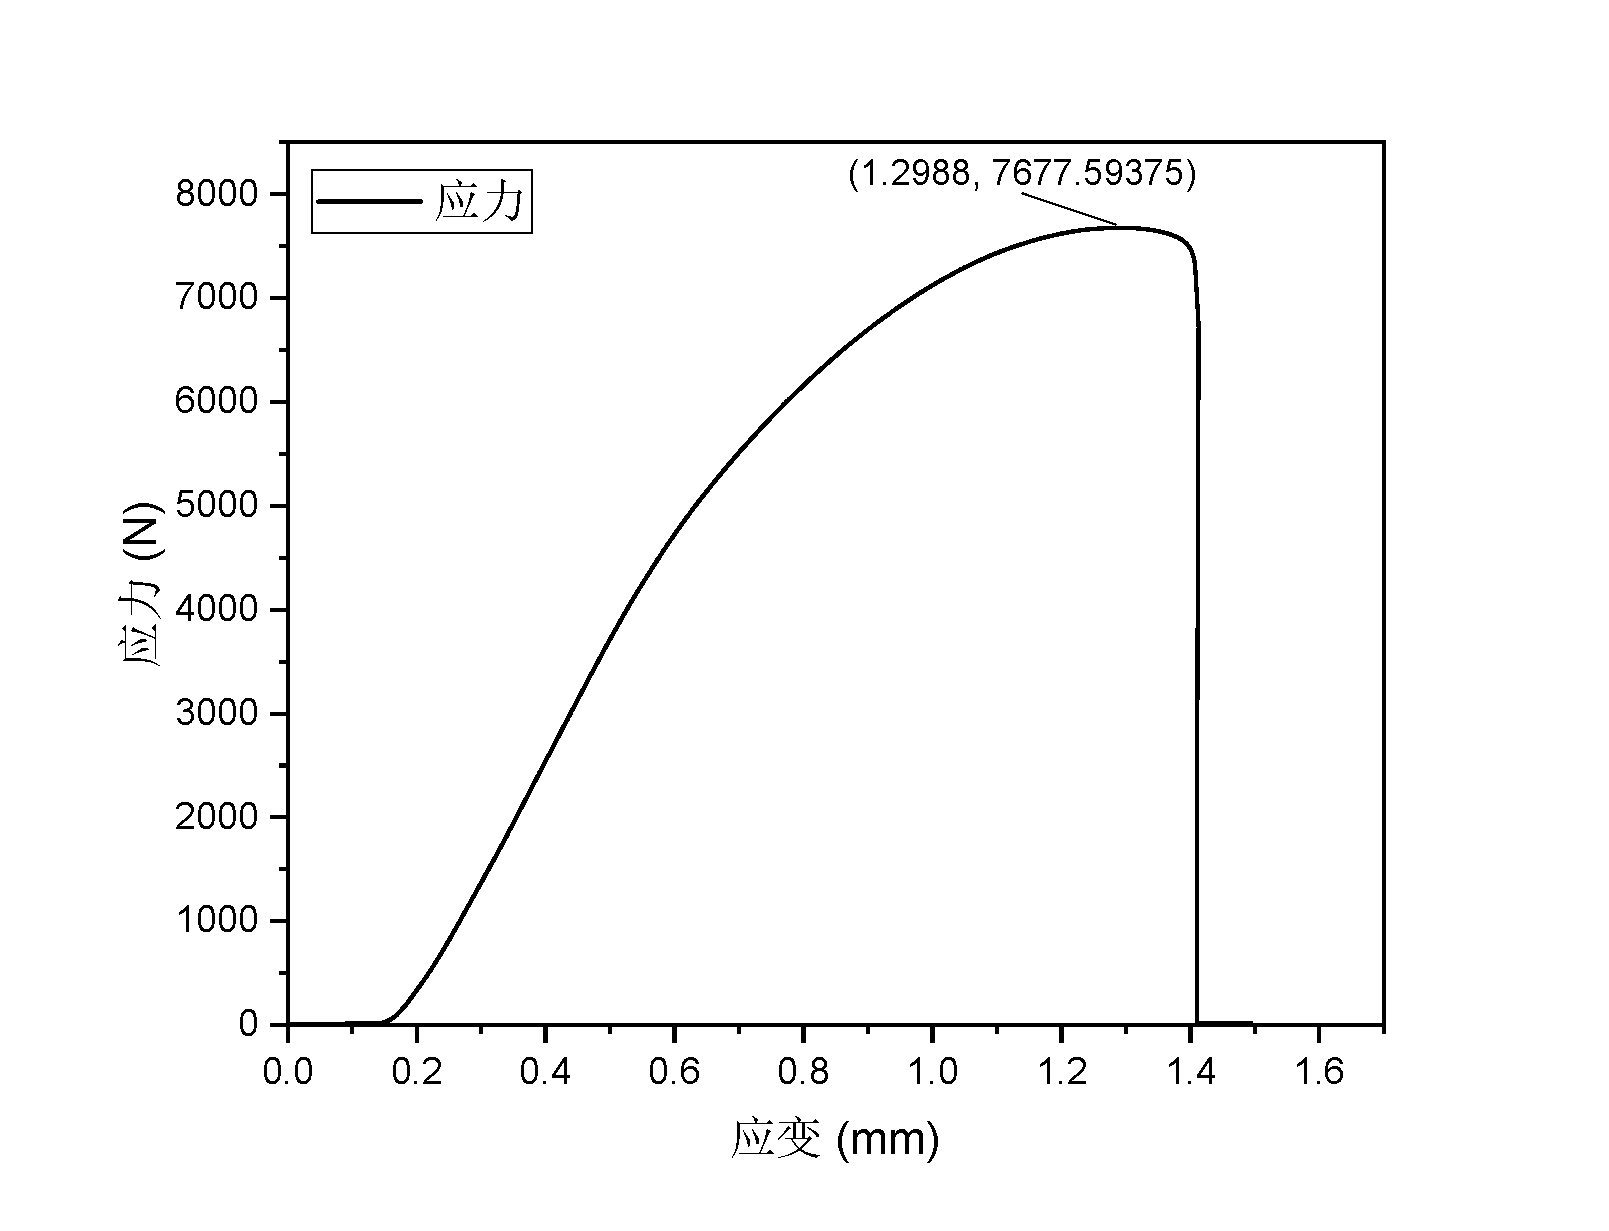
\includegraphics[width=0.5\textwidth]{img/A6/ironPush.pdf}
    \end{figure}

    \subsection{数据计算}
    \noindent 低碳钢强度极限
    \begin{equation}
        \sigma_1=\frac{F_1}{S_{1}}=\frac{4 F_1}{\pi d_{0}^2}=\frac{4\times 4456.21924}{\pi(3.89\times 10^{-3})^{2}}=\SI{3.74954d8}{\Pa}
    \end{equation}
    铸铁强度极限
    \begin{equation}
        \sigma_2=\frac{F_2}{S_{2}}=\frac{4 F_2}{\pi d_{0}^2}=\frac{4\times  7677.59375}{\pi(3.88\times 10^{-3})^{2}}=\SI{6.49339d8}{\Pa}
    \end{equation}
\section{结果分析}
    \subsection{数据分析}
        \begin{enumerate}
            \item 实验计算的低碳钢的名义屈服强度为 \SI{374.954}{\MPa},与理论值 \SI{207}{\MPa} 的相对误差极大。查阅资料得知,可能是因为低碳钢的名义屈服强度会随着含碳量和试件高度而改变,以及可能有摩擦力等因素的影响。
            \item 实验计算的铸铁的强度极限为 \SI{649.339}{\MPa},查阅文献可以知道强度极限参考值在\linebreak 602-\SI{700}{\MPa},实验测量结果处于范围之内。
            \item 初始阶段材料几乎服从胡克定律。但当载荷达到一定值以后,我们可以从低碳钢压缩曲线图看出,随载荷增加,曲线不再为线性,但试样无明显屈服现象。随载荷进一步增大,曲线增长速度减缓。这是因为随着塑性变形的迅速增长,试样横截面积逐渐增大,增加了承载能力,使变形速度下降。而从铸铁压缩曲线可以看出,铸铁在达到强度极限后直接被破坏,这是因为被压缩时试样受压时将沿与轴线成 $45^\circ$-$55^\circ$ 倾角的斜截面发生错动,而且铸铁的微观结构中含有大片石墨和脆性相,以及铸铁的晶粒较大且不均匀,晶界处容易集中应力,使铸铁在压缩过程中发生断裂。
        \end{enumerate}
    \subsection{误差分析}
    \subsubsection{系统误差}
    \begin{enumerate}
        \item 环境:实验当天的温度、湿度所带来的误差。查阅资料得知,温度、湿度会在一定程度下影响材料的力学性质,进而影响实验测量。
        \item 仪器:诸如测量数据时的精度,加载应力时的均匀程度之类仪器本身的误差,以及用游标卡尺测量直径和长度时精度带来的误差。
        \item 试样:不同的试样中的组成成分差异带来的误差。
    \end{enumerate}
    \subsubsection{偶然误差}
    \begin{enumerate}
        \item 读数:在用游标卡尺测量试样的长度和直径时,可能会由于估读而产生读取数据的误差。
        \item 计算:在对数据进行处理分析时,可能会由于四舍五入而产生计算的误差。
    \end{enumerate}
\section{思考题}
\begin{enumerate}
    \item \thinking{试分析低碳钢和铸铁试件在压缩过程中及破坏后有哪些区别。}{%
    低碳钢和铸铁在压缩过程中及破坏后有许多区别,主要包括以下几个方面:
    \begin{enumerate}
        \item 形变行为:在压缩加载下,低碳钢通常会表现出更多的塑性变形能力,可以发生较大的塑性变形,而铸铁的塑性较差,容易出现脆性断裂。
    
        \item 破坏形态:低碳钢在受到压缩力作用时,通常会发生均匀的塑性变形,最终可能会出现局部的颈缩现象,但整体上会保持一定的连续性;而铸铁在受到压缩力作用时,由于其较差的塑性,容易在应力集中的区域发生裂纹扩展,最终可能呈现出明显的断裂表面。
    
        \item 应力应变曲线:低碳钢在压缩加载下的应力应变曲线通常会比较平缓,在达到极限强度前会有明显的应变硬化阶段;而铸铁的应力应变曲线往往会比较陡峭,在达到极限强度前可能会表现出较少的应变硬化。
    
        \item 能量吸收能力:由于低碳钢具有较好的塑性,因此在压缩过程中能够吸收较多的变形能量,而铸铁的能量吸收能力较低。
    
        \item 微观结构变化:低碳钢在压缩加载过程中,晶粒可能会发生滑移和再结晶等变化,而铸铁中的石墨颗粒会对应力分布产生影响,导致其微观结构的变化。
    \end{enumerate}
    综上所述,低碳钢和铸铁在压缩过程中及破坏后的表现有很大的区别,主要表现在塑性、破坏形态、应力应变曲线、能量吸收能力和微观结构变化等方面。}
    \item \thinking{与拉伸实验相比较,分析低碳钢和铸铁在压缩时的破坏原因。}{%
    低碳钢在压缩过程中,低碳钢通常会表现出更多的塑性变形能力。当受到压缩力时,钢材会发生塑性变形,晶粒会发生滑移和再结晶,使得材料可以更充分地吸收能量。低碳钢在压缩时的破坏通常是由于材料内部的局部应力集中导致的,可能会出现塑性变形过大、局部失稳等情况,最终导致材料的断裂。相比之下,铸铁在压缩时通常会表现出更脆的特性。铸铁的微观结构中含有大量的石墨片或球状石墨,这些石墨会成为应力集中的点,导致材料容易发生裂纹。因此,铸铁在受到压缩力作用时,容易出现裂纹扩展和断裂,而不像低碳钢那样具有较强的塑性变形能力。}
    \item \thinking{为什么低碳钢压缩时测不出强度极限?}{%
    低碳钢延展性强,载荷虽然不断增加,但试件只是被压扁而并未被破坏,即便被压成饼状也不会断裂,因此无法求出强度极限。}
    \item \thinking{简述低碳钢和铸铁的力学性能的主要区别。}{%
    低碳钢具有良好的塑性和延展性,抗拉强度和屈服强度相对较高,但相对硬度较低。适用于需要强度和韧性兼备的场合,如结构件、机械零件等。而铸铁具有较高的硬度和耐磨性,但延展性较差,容易发生脆性断裂。常用于制造需要抗压、耐磨的零件,如汽车发动机缸体、机械床身等}
\end{enumerate}
